\documentclass{article}
\usepackage{lipsum}
\usepackage{amsmath, mathrsfs, amsfonts}
\usepackage{tikz}
\usepackage{graphicx}



\begin{document}
    \centering
    Hello world!
    \[ a^2 + b^2 = c^2 + d^2 \]
    Goodbye.

    \begin{figure}[htbp]
        \centering
        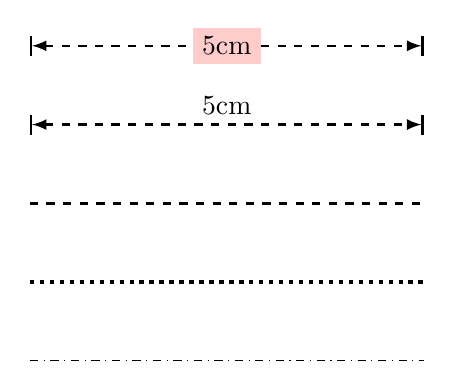
\begin{tikzpicture}[>=latex]  % 放在 begin 后边的是宏操作;箭头类型还有 stealth
            \draw[|<->|, dashed, thick] (0, 0)--node[above]{5cm}(5, 0);
            % node 结点 ,above, below, right, left, "=3mm":调整结点位置
            % node 在谁的后边,图上结点就在对应的位置
            
            \draw[|<->|, dashed, thick] (0, 1)--node[fill = red!20!white]{5cm}(5, 1);
            % xcolor 的宏包可以实现颜色调配;"red!20!white" 是百分之20的红色加上百分之80的白色
            
            \draw[dashed, very thick] (0, -1) to (5, -1);
            \draw[dotted, ultra thick] (0, -2) to (5, -2);
            \draw[dashdotted, thin] (0, -3) to (5, -3);
        \end{tikzpicture}
        \caption{}
    \end{figure}


    \begin{figure}[htbp]
        \centering
        \begin{tikzpicture}[>=latex]
            \draw[->] (-1, 0) -- (4, 0)node[below]{$x$};
            \draw[->] (0, -1) -- (0, 4)node[left]{$y$};
            \draw (0, 2)node[left]{$N$} -- (2, 2)node[right]{$P(x,y)$} -- (2, 0)node[below]{$M$};
            \node at (-.2, -.2){$O$};   %"\node at" 在某一点写入文本
            \draw (1, 0)node[below]{$1$} -- (1, .1);
            \draw (0, 1)node[left ]{$1$} -- (.1, 1);

        \end{tikzpicture}

    \end{figure}


    \begin{figure}[htbp]
        \centering
        \begin{tikzpicture}[>=latex]
            \draw[->] (-1, 0) -- (4, 0)node[below]{$x$};
            \draw[->] (0, -1) -- (0, 4)node[left ]{$y$};
            \foreach \c in {1, 2, 3}
            {
                \draw[thick] (0, \c)node[left ]{$\c$} -- (.1, \c);
                \draw[thick] (\c, 0)node[below]{$\c$} -- (\c, .1);
                \foreach \b in {1, 2, ..., 9}
                {
                    \draw[thin] (0, \c - \b*0.1) -- (.05, \c - \b*0.1);
                    \draw[thin] (\c - \b*0.1, 0) -- (\c - \b*0.1, .05);
                }
            }
        \end{tikzpicture}
    
    \end{figure}
    
    \end{document}

\end{document}



